% Dokumentklassen:
% article, report, beamer, book, letter etc.
% https://en.wikibooks.org/wiki/LaTeX/Document_Structure
\documentclass[a4paper]{article}

% Seitenränder Abstand setzen
\usepackage[margin=80pt]{geometry}

% Deutsches Sprachpaket
\usepackage[ngerman]{babel}
% UTF8 Input Encoding
\usepackage[utf8]{inputenc}

% Schriftbild ändern
% https://en.wikibooks.org/wiki/LaTeX/Fonts
\usepackage[scaled]{helvet}
% (Sans) Serifen oder anderes
% \rmdefault: Serifen
% \sfdefault: Sans-Serifen
% \ttdefault: Typewriter
\renewcommand{\familydefault}{\sfdefault}
% Fontencoding (für ä, ö, ü etc.)
\usepackage[T1]{fontenc}

% Gänsefüsschen richtig kompilieren
\usepackage [autostyle]{csquotes}
\MakeOuterQuote{"}

% Hyperlinks farblos
\usepackage[hidelinks]{hyperref}
\hypersetup{colorlinks=false}

% Package für Aufzählungen
\usepackage{enumitem}
% kein Abstand zwischen Aufzählungen
% Sollen doch Abstände vorhanden sein: nach Aufzählung {itemsep=1em}
\setlist{nosep}

% Grafik-Packages, für Figures, Subfigures und PDF als Import
\usepackage{graphicx}
\usepackage{subcaption}
\usepackage{pdfpages}

% Package und Einstellungen für Java-Code-Darstellung
% Werden erstellt mit \begin{lstlisting}
\usepackage{listings}
\usepackage{color}
\definecolor{dkgreen}{rgb}{0,0.6,0}
\definecolor{gray}{rgb}{0.5,0.5,0.5}
\definecolor{mauve}{rgb}{0.58,0,0.82}
\lstset{frame=tb,
	language=Java,
	aboveskip=3mm,
	belowskip=3mm,
	showstringspaces=false,
	columns=flexible,
	basicstyle={\small\ttfamily},
	numbers=none,
	numberstyle=\tiny\color{gray},
	keywordstyle=\color{blue},
	commentstyle=\color{dkgreen},
	stringstyle=\color{mauve},
	breaklines=true,
	breakatwhitespace=true,
	tabsize=3
}

\title{\textbf{DL4G - Questionnaire} \\
Deep Learning for Games}
\date{\today}
\author{Maurin D. Thalmann}

\begin{document}
	
	\pagenumbering{gobble}
	\maketitle
	
	\begin{center}
		Dieser Questionnaire wurde basierend auf einer Card2Brain Sammlung erstellt:  \\
		\href{https://card2brain.ch/box/20190124_dl4g}{Card2Brain - DL4G} (Credits: Cyrille Ulmi)
	\end{center}
	
	\newpage
	\pagenumbering{arabic}
	\tableofcontents
	
	\newpage
	
	\section{Sequenzielle Spiele}
	
		\subsection{Was sind die Eigenschaften von endlichen-sequenziellen Spielen?}
		
		\begin{itemize}
			\item Eine endliche Anzahl Spieler mit einer endlichen Anzahl Aktionen
			\item Die Aktionen werden sequenziell ausgewählt
			\item Es wird eine endliche Anzahl Runden gespielt
			\item Spätere Spieler sehen die Aktionen vorheriger Spieler
		\end{itemize}
	
		\subsection{War wird unter Perfect Recall verstanden?}
		
		Perfekte Erinnerung an alle vorherigen Züge
		
		\subsection{Was ist eine Strategie?}
		
		Sagt einem Spieler, welche Aktion im aktuellen Zug auszuführen ist
		
		\subsection{Was ist ein Strategie-Profil?}
		
		Die ausgewählte Strategie eines Spielers
		
		\subsection{Was ist eine Utility- oder Payoff-Function?}
		
		Sie berechnet das Resultat für jede Aktion
		
		\subsection{Was sind die Komplexitätsfaktoren bei einer Spielanalyse?}
		
		\begin{itemize}
			\item Anzahl Spieler
			\item Grösse des Suchraums (Anzahl gespielte Züge \& Anzahl mögliche Aktionen)
			\item Kompetitiv vs. Kooperativ
			\item Stochastische Spiele (mit Zufall) vs. Deterministisch
			\item Perfekte vs. imperfekte Information
		\end{itemize}
	
		\subsection{Was ist imperfekte Information?}
		
		\begin{itemize}
			\item Das Spiel konnte nur teilweise beobachtet werden
			\item Man kennt bspw. nicht die Karten der anderen Spieler
		\end{itemize}
	
		\subsection{Beispiele von Spielen mit perfekten / imperfekten Informationen?}
		
		Perfekt (Schach) und imperfekt (Jass, Poker)
		
		\subsection{Was ist der Suchraum?}
		
		Anzahl gültige Brettpositionen und die untere Grenze des Suchbaums
		
		\subsection{Was ist ein Suchbaum?}
		
		\begin{itemize}
			\item Knoten sind Spielpositionen / Spielzustände
			\item Kanten sind Aktionen / Spielzüge
			\item Blätter werden durch Payoff-Funktionen definiert
		\end{itemize}
	
		\subsection{Wie funktioniert Backward Induction?}
		
		\begin{itemize}
			\item Den Baum von unten nach oben durcharbeiten (bzw. von rechts nach links)
			\item Immer den besten Weg für den aktuellen Spieler markieren
			\item Geeignet für sequenzielle endliche Spiele mit perfekter Information
		\end{itemize}
		
		\subsection{Was bedeutet Rationalität?}
		
		Dass der Spieler nicht die schlechtere Alternative wählt
		
		\subsection{Welche Arten von Lösungen werden bei endlich-sequenziellen Spielen unterschieden?}
		
		\begin{itemize}
			\item Ultra-schwache Lösung
			\begin{itemize}
				\item Bestimmt, ob der erste Spieler einen Vorteil aus der Initialposition hat, ohne die genaue Strategie zu kennen
				\item Setzt perfektes Spielen des Gegners voraus
				\item Beispielsweise durch Existenzbeweise in der Mathematik
			\end{itemize}
			\item Schwache Lösung
			\begin{itemize}
				\item Kann ein komplettes Spiel mit perfekten Zügen aus der Initialposition durchspielen
				\item Geht von einem perfekten Spiel des Gegners aus
			\end{itemize}
			\item Starke Lösung
			\begin{itemize}
				\item Kann aus jeder Position heraus perfekte Züge spielen
				\item Kann auch gewinnen, wenn vorherige Spieler einen Fehler gemacht haben
			\end{itemize}
		\end{itemize}
		
		\subsection{Was versteht man unter einem Zero-Sum Game (Nullsummenspiel)?}
		
		\begin{itemize}
			\item Der Vorteil für einen Spieler ist zum Nachteil des anderen Spielers
			\item Die Punktesumme für zwei Strategien ist immer gleich Null
		\end{itemize}
	
		\subsection{Was sind Charakteristiken des Minimax-Algorithmus?}
		
		\begin{itemize}
			\item Gilt nur für ein Nullsummenspiel
			\item Zwei Möglichkeiten / Ziele
				\begin{itemize}
					\item den eigenen Gewinn maximieren
					\item den Gewinn des Gegners minimieren
				\end{itemize}
		\end{itemize}
	
		\subsection{Wie funktioniert der Minimax-Algorithmus?}
		
		\begin{itemize}
			\item Wenn der Knoten mir gehört: Aktion wählen, die den Payoff maximiert
			\item Wenn der Knoten dem Gegner gehört: Aktion wählen, die den Payoff minimiert
			\item Wenn es ein Endknoten ist: den Payoff berechnen
		\end{itemize}
	
		\subsection{Was versteht man unter Search Tree Pruning?}
		
		Nicht relevante Teilbäume können weggelassen werden, reduziert den Rechenaufwand
		
		\subsection{Was sind die Regeln von Alpha-Beta Pruning?}
		
		\begin{itemize}
			\item $\alpha$ ist der grösste Wert alles MAX Vorfahren eines MIN Knoten
			\item $\beta$ ist der kleinste Wert alles MIN Vorfahren eines MAX Knoten
			\item Den Teilbaum abschneiden, falls er grösser als $\alpha$ oder kleiner als $\beta$ ist
		\end{itemize}
		
		\subsection{Was ist der Vorteil von Alpha-Beta Pruning?}
		
		\begin{itemize}
			\item $b$ = Anzahl Kanter der Knoten und $m$ = Tiefe des Baums
			\item Ordnung verbessert sich von $O(b^{m})$ nach $O(b^{m/2})$, halbiert also die Tiefe der Suchbäume
		\end{itemize}
	
	\section{Monte Carlo Tree Search}
	
		\subsection{Wieso werden Random Walks eingesetzt? (Tree Search)}
		
		\begin{itemize}
			\item Der Suchraum ist oft zu gross für eine vollständige Suche
			\item Die Idee, verglichen zu Minimax, ist, bei einer bestimmten Tiefe zu stoppen und zu raten
		\end{itemize}
		
		\subsection{Was ist die Idee hinter Monte Carlo Tree Search?}
		
		\begin{itemize}
			\item Macht einen Random Walk und spielt zufällige Simulationen
			\item Versucht, in einer fixen Zeit möglichst viel des Suchraums zu entdecken
			\item Am Schluss wird der vielversprechendste Spielzug ausgewählt
		\end{itemize}
	
		\subsection{Welche 4 Phasen gibt es bei Monte Carlo Tree Search?}
		
		\begin{enumerate}
			\item \textbf{Selection}
			\begin{itemize}
				\item Starte beim Wurzelknoten \texttt{R} und wähle fortlaufend Kinderknoten
				\item Stoppe, wenn du einen Knoten erreichst, der noch nicht komplett erweitert/erforscht wurde
				\item Benötigt ein Kriterum für die Auswahl der Kinderknoten, sogennante \textit{tree policy}
			\end{itemize}
			\item \textbf{Expansion}
			\begin{itemize}
				\item Wenn das Zeitlimit \texttt{L} das Spiel beendet, gib die Payoffs zurück
				\item Sonst, wähle eine unerforschte Aktion und kreiere einen Knoten \texttt{C} für diese
			\end{itemize}
			\item \textbf{Simulation}
			\begin{itemize}
				\item Simuliere ein Weiterspielen von Knoten \texttt{C} aus, mithilfe einer \textit{default policy}
				\item Im simpelsten Fall, spiele einfach bis zu irgendeinem Ende mit zufälligen Zügen
			\end{itemize}
			\item \textbf{Backpropagation}
			\begin{itemize}
				\item Aktualisiere die gespeicherten Informationen in jedem Knoten von \texttt{C} zurück bis zu \texttt{R}
				\item MCTS erwartet einen Payoff in [0,1]
			\end{itemize}
		\end{enumerate}
	
		\subsection{Welche zwei Ansätze gibt es beim Auswählen eines neuen Knotens?}
		
		\begin{itemize}
			\item Exploitation
			\begin{itemize}
				\item Immer den besten Payoff wählen
				\item Anhand von Beobachtungen auf der besten Maschine spielen, um Gewinn zu maximieren
			\end{itemize}
			\item Exploration
			\begin{itemize}
				\item Etwas Neues wählen, versuchen möglichst viel zu erkunden
				\item Alle Maschinen spielen, um möglichst viel Informationen zu gewinnen
			\end{itemize}
		\end{itemize}
	
		\subsection{Was ist die Idee hinter UCB1 (Upper Confidence Bound)?}
		
		\begin{itemize}
			\item Die beste Strategie ist eine Mischung aus Exploitation und Exploration
			\item Ergibt ein statistisches Konfidenzintervall für jede Option
			\item Parameter $c$ kontrolliert den Trade-Off zwischen Exploitation und Exploration
		\end{itemize}
	
		\subsection{Was ist sehr wichtig bei der Anwendung von UCB1?}
		
		Immer die Vektor-Komponente des aktuellen Spielers für die Berechnung verwenden.
		
		\subsection{Was passiert bei MCTS, wenn die Zeit abgelaufen ist?}
		
		Spielt die Aktion mit der höchsten Anzahl an Besuchen.
		
		\subsection{Was sind Unterschiede zwischen Minimax und MCTS?}
		
		\begin{itemize}
			\item Beide Algorithmen setzen perfekte Informationen voraus
			\item Minimax ist nur anwendbar auf Nullsummenspiele mit zwei Spielern
			\item MCTS funktioniert für jedes Spiel mit perfekter Information
			\item Minimax optimiert Payoffs, MCTS optimiert einen Exploitation-Exploration Trade-Off
			\item MCTS ist ein Anytime-Algorithmus, Minimax nicht
			\item Monte Carlo Bäume sind asymmetrisch, Minimax Bäume sind symmetrisch
		\end{itemize}
		
		\subsection{Was ist ein Anytime-Algorithmus?}
		
		Er kann eine gültige Lösung zurückgeben, auch wenn die Ausführung vorzeitig abgebrochen wird.
		Es wird erwartet, dass er eine immer bessere Lösung findet, je länger er ausgeführt wird.
		
		\subsection{Wie sehen die Payoffs bei MCTS aus und was wird maximiert?}
		
		\begin{itemize}
			\item Für ein Beispiel mit 2 Spielern nimmt der Payoff-Vektor die Form $(W, N-W)$ an
			\item Spieler 1 maximiert $W$, Spieler 2 maximiert $N-W$ (implizit minimiert Spieler 2 so auch $-W$)
		\end{itemize}
	
	\section{Information Sets}
	
		\subsection{Was ist ein Information Set?}
		
		\begin{itemize}
			\item Ein Information Set ist eine Menge von Knoten des gleichen Spielers
			\item Der Spieler kennt den vorherigen Zug nicht
			\item Alle Knoten müssen die gleichen Optionen bieten
			\item Sind immer aus der Sicht eines Spielers
		\end{itemize}
	
		\subsection{Was ist der Unterschied zwischen perfekter und imperfekter Information?}
		
		\begin{itemize}
			\item Unterschiedliche Strategien werden gewählt
			\item Bei perfekter Information hat jeder Knoten exakt eine Option
		\end{itemize}
	
		\subsection{Was ist die Idee hinter Determinization?}
		
		\begin{itemize}
			\item Unbekannte Karten zufällig auf die Gegner verteilen
			\item Danach das Anwenden der Regeln von perfekter Information (bspw. mit MCTS)
			\item Ergibt dann mehrere mögliche Suchbäume
			\item Schlussendlich über alle Bäume die Option wählen, die am meisten besucht wurde
			\item Manchmal werden Entscheidungen getroffen, welche gar nie eintreten können, was zu falschen Entscheidungen führen kann
		\end{itemize}
	
		\subsection{Was muss bei einer Implementation von MCTS mit Information Sets beachtet werden?}
		
		\begin{itemize}
			\item Der Baum besteht aus Information Sets und nicht mehr aus Zuständen
			\item Knoten entsprechen Information Sets aus der Sicht des Wurzelspielers
			\item Karten werden zufällig verteilt und ungültige Varianten werden ausgeblendet
			\item Kanten entsprechen einer Aktion, welche in mindestens einem Zustand möglich ist
			\item Funktioniert danach wie ein Spiel mit perfekter Information
		\end{itemize}
	
		\subsection{Wie muss die UCB1 angepasst werden für Information Sets?}
		
		\begin{itemize}
			\item $N_{p}$ = Anzahl Besuche des Vorgänger-Knotens und wie oft Knoten $i$ verfügbar war
			\item Knotenliste ergänzen um "wie viel mal war jede Option verfügbar"
		\end{itemize}
	
	\newpage
	
	\section{Supervised Machine Learning}
	
		\subsection{Welche Disziplinen gibt es bei Machine Learning?}
		
		\begin{itemize}
			\item Supervised Learning
			\begin{itemize}
				\item Dem Algorithmus werden gelabelte Trainingsdaten übergeben
				\item Er lernt, Labels von unbenannten Daten vorherzusagen
			\end{itemize}
			\item Unsupervised Learning
			\begin{itemize}
				\item Dem Algorithmus werden nicht gelabelte Trainingsdaten übergeben
				\item Er entdeckt / lernt selbstständig die Struktur der Daten
			\end{itemize}
			\item Semi-Supervised Learning
			\begin{itemize}
				\item Mischung zwischen Supervised und Unsupervised Learning
				\item Wird meist benutzt, wenn eine kleine Anzahl gelabelter Daten zur Verfügung steht
			\end{itemize}
			\item Reinforcement Learning
			\begin{itemize}
				\item Keine Daten stehen zur Verfügung
				\item Der Algorithmus wird durch eine Reward Funktion geleitet
				\item Das ideale Verhalten wird gesucht, um die Reward Funktion zu maximieren
			\end{itemize}
		\end{itemize}
		
		\subsection{Was können die Gründe für schlechte Datenqualität sein?}
		
		\begin{itemize}
			\item Schlechtes Design, mangelhafte oder inkonsistente Datenformate
			\item Programmierfehler oder technische Probleme
			\item Alter der Daten (bspw. ungültige E-Mail-Adressen)
			\item Schlechte Dateneingabemasken (fehlende Validierung bei Erfassung der Daten)
			\item Menschliche Fehler beim Datenexport
			\item Ungültige oder falsche Informationen
		\end{itemize}
	
		\subsection{Welche Möglichkeiten gibt es, um die Qualität von Daten festzustellen?}
		
		\begin{itemize}
			\item Datenquellen und deren Zuverlässigkeit überprüfen
			\item Statistische Kennzahlen interpretieren und überprüfen
			\item Visuelles Überprüfen eines Datenauszugs
			\item Manuell Datenbereiche überprüfen (bspw. negative Löhne)
			\item Plausibilität von Zusammenhängen überprüfen
			\item Redundanz der Daten messen
			\item Abweichungen in Syntax und Semantik der Daten
			\item NULL-Werte und doppelte Daten untersuchen
		\end{itemize}
		
		\subsection{Wie läuft ganz einfaches Machine Learning ab?}
		
		\begin{itemize}
			\item Daten in Testdaten und Trainingsdaten aufteilen
			\item Klassifikator auf den Trainingsdaten trainieren
			\item Klassifikator anhand der Testdaten bewerten
		\end{itemize}
		$\rightarrow$ Funktioniert nur mit vielen Daten und wenn die Hyperparameter festgelegt sind
		
		\subsection{Wie sollten die Daten in einem Date Pool aufgeteilt werden?}
		
		\begin{itemize}
			\item ca. 70-80\% Trainingsdaten
			\item ca. 20-30\% Testdaten
		\end{itemize}
	
		\subsection{Wie sollte beim Aufteilen der Daten vorgegangen werden?}
		
		\begin{itemize}
			\item Daten zufällig mischen
			\item Daten aufteilen in Training und Test
			\item Training- und Testdaten müssen disjunkt sein (keine gemeinsamen Elemente)
		\end{itemize}
		
		\subsection{Was bedeutet Training? (ML)}
		
		Minimierung einer Kostenfunktion auf den Trainingsdaten durch Anpassen der Modellparameter
		
		\subsection{Was bedeutet Testing? (ML)}
		
		Nur eine Auswertung auf unbekannten Daten ermöglicht, die Leistung eines Modells festzustellen
		
		\subsection{Was ist k-NN?}
		
		\begin{itemize}
			\item Steht für K-Nearest Neighbors
			\item Ist ein sehr einfacher Machine-Learning-Algorithmus
			\item Bei $k=1$ wird das Label des nächstgelegenen Trainingspunkt verwendet
			\item Bei $k>1$ findet ein Mehrheitsbeschluss der nächsten $k$ Nachbarn statt
		\end{itemize}
		
		\subsection{Was sind Hyperparameter?}
		
		\begin{itemize}
			\item Entscheidungen, die vom Menschen getroffen werden
			\item Zum Beispiel: Angleichung an eine lineare Funktion
		\end{itemize}
	
		\subsection{Was sind Beispiele für Hyperparameter?}
		
		\begin{itemize}
			\item Anzahl Nachbarn bei k-NN
			\item Regularisierung der Parameter
			\item Kernel einer Support-Vektoren-Maschine
			\item Baumtiefe und Selection-Policy im Entscheidungsbaum
			\item Anzahl Layers, Neuronen, Aktivierungsfunktion, Dropout bei Deep Learning
		\end{itemize}
	
		\subsection{Wie sieht ein komplizierter Auswertungsvorgang aus? (ML)}
		
		\begin{itemize}
			\item Daten aufteilen in 60\% Training, 20\% Validation und 20\% Test
			\item Über alle interessanten Hyperparameter-Konfigurationen iterieren
			\item Modell anhand der ausgewählten Hyperparameter auf den Trainingsdaten trainieren
			\item Modell auf dem Validation-Set überprüfen und Leistung messen
			\item Modell mit der besten Leistung auswählen und auf den Testdaten Leistug messen
		\end{itemize}
		$\rightarrow$ Diese variante benötigt ziemlich viele Daten
		
		\subsection{Was ist das Ziel von Cross Validation?}
		
		\begin{itemize}
			\item Falls zu wenig Daten vorhanden sind
			\item Aufteilen in 80\% Training und 20\% Test
			\item Training aufteilen in $k$ Folds (bspw. 10)
			\item Jeder Fold ist einmal das Validation-Set
			\item Die restlichen Folds werden als Trainingsdaten verwendet
			\item Schlussendlich den Mittelwert über alle Folds ziehen
		\end{itemize}
	
		\subsection{Was ist das Ziel bei Aufteilung in Test- und Trainings-Set?}
		
		Gleiche Verteilungen über Test- und Trainings-Set
		
		\subsection{Was sollte man über Learning-Curves wissen?}
		
		\begin{itemize}
			\item Wenn Kurven weit auseinander sind, hilft es wenn man mehr Daten nutzt
			\item Wenn Kurven parallel sind, dann bringt es ziemlich sicher nichts
		\end{itemize}
	
	\newpage
	
		\subsection{Welche Möglichkeiten gibt es bei einer Confusion Matrix für einen Binary Classifier?}
		
		\begin{description}
			\item[TN] = true-negative
			\item[FP] = false-positive
			\item[FN] = false-negative
			\item[TP] = true-positive
		\end{description}
	
		\begin{table}[]
			\begin{tabular}{|l|l|l|}
				\hline
				\textbf{Vorhersage}       & \textbf{Wahr} & \textbf{Falsch} \\ \hline
				\textbf{Realität: \textit{Wahr}}   & TP            & FN              \\ \hline
				\textbf{Realität: \textit{Falsch}} & FP            & TN              \\ \hline
			\end{tabular}
		\end{table}
	
		\subsection{Wie werden Accuracy und Error Rate berechnet?}
		
		\begin{itemize}
			\item Accuracy = $\frac{TP + TN}{Total}$\\
			\item Error Rate = $\frac{FP + FN}{Total} = 1 - Accuracy$
		\end{itemize}
	
	\section{Neuronal Networks}
	
		\subsection{Was ist der Unterschied zwischen AI und Deep Learning?}
		
		\begin{itemize}
			\item Artificial Intelligence (regelbasiert / MCTS)
			\item Machine Learning (Training auf Daten mit festgelegten Features)
			\item Deep Learning (Lernen der Features aus den Daten)
		\end{itemize}
	
		\subsection{Was ist die Definition von Machine Learning?}
		
		\begin{itemize}
			\item Ein Computerprogramm \textbf{lernt} aus der Experience $E$...
			\item ...mit Rücksicht auf eine Klasse von Tasks $T$ und Performance Measures $P$...
			\item ...wenn es Tasks in $T$ durchführt, gemessen an $P$, seine Experience $E$ verbessert.
		\end{itemize}
	
		\subsection{Was ist $T$ beim Jassen? (ML)} 
		
		Tasks ($T$)
		\begin{itemize}
			\item Trumpf auswählen
			\item Karte auswählen
			\item Werte der Karten
			\item Punkte im Spiel
		\end{itemize}
	
		\subsection{Was ist $P$ beim Jassen? (ML)}
		
		Performance Measure ($P$)
		\begin{itemize}
			\item Anzahl Gewinne / Punkte
			\item Vergleich mit Daten
		\end{itemize}
		
		\subsection{Was wäre $E$ beim Jassen? (ML)}
		
		Experience ($E$)
		\begin{itemize}
			\item Spielen
			\item Daten lesen
		\end{itemize}
		
		\subsection{Welche zwei Task-Typen werden unterschieden? (ML)}
		
		Regression \& Classification
		
		\subsection{Aus welchen 3 Teilen besteht ein Feed Forward Network?}
		
		\begin{itemize}
			\item Input Layer
			\item Hidden Layer
			\item Output Layer
		\end{itemize}
	
		\subsection{Was beinhaltet ein Knoten eines Netzwerks?}
		
		\begin{itemize}
			\item Inputs ($x_{1}$, $x_{2}$, ...)
			\item Internen Parameter ($\Theta$)
			\item Funktion, die den Output basierend auf dem Parameter berechnet
		\end{itemize}
	
		\subsection{Was ist eine Epoche?}
		
		Ein (1) Training des gesamten Datensets
		
		\subsection{Welche Aktivierungsfunktionen gibt es?}
		
		\begin{itemize}
			\item Sigmoid für eine binäre Klassifizierung
			\item relu für Nodes innerhalb eines Netzwerks
			\item Aktivierungsfunktion sollte nicht linear sein
		\end{itemize}
	
		\subsection{Was ist eine Kostenfunktion?}
		
		\begin{itemize}
			\item Ist die Funktion, welche durch das Lernen minimiert werden soll
			\item Häufig wird eine Likelihood-Funktion verwendet
		\end{itemize}
	
		\subsection{Was sollte bei Multi-Class Problemen beachtet werden?}
		
		\begin{itemize}
			\item 1-hot encoded Array für Labels
			\item Letzter Layer mit softmax Funktion (für Normierung)
		\end{itemize}
	
		\subsection{Was ist ein neuronales Netzwerk?}
		
		\begin{itemize}
			\item Besteht aus mathematischen Knoten
			\item Knoten haben Inputs und Outputs
			\item Knoten sind organisiert in Layers
			\item Knoten berechnen aus Inputs und Parameter einen Output
			\item Knoten haben lineare Funktion (Gewicht, Bias, Input)
			\item Auf Funktion wird eine Aktivierungsfunktion angewendet (sigmoid, relu)
		\end{itemize}
	
		\subsection{Wie berechnet ein neuronales Netzwerk das Resultat?}
		
		\begin{itemize}
			\item Parameter werden während dem Training definiert
			\item Danach nur noch Layer für Layer durchrechnen
		\end{itemize}
	
		\subsection{Was ist eine Loss Funktion?}
		
		\begin{itemize}
			\item Grundsätzlich eine Fehlerfunktion
			\item Die Funktion, welche während dem Training minimiert werden soll
		\end{itemize}
		
		\subsection{Wie wird ein neuronales Netzwerk trainiert?}
		
		\begin{itemize}
			\item Differenz zwischen berechnetem Wert und gegebenem Label
			\item Es wird versucht, Differenzen zu minimieren
		\end{itemize}
	
		\subsection{Wie kann das Training auf seine Wirksamkeit überprüft werden?}
		
		\begin{itemize}
			\item Benötigt eine Metrik und Testdaten
			\item Zum Beispiel: Überprüfen der Accuracy
		\end{itemize}
	
		\subsection{Was ist der Vorteil eines Deep Neuronal Networks?}
		
		Features werden automatisch berechnet
		
		\subsection{Was ist das Problem mit der optimalen Kapatität? (NN)}
		
		\begin{itemize}
			\item Mit mehr Trainingsdaten wird der Fehler kleiner
			\item Der Fehler der Testdaten wird dann jedoch immer grösser
		\end{itemize}
	
		\subsection{Welche 3 Klassen gibt es bei VOC Challenges?}
		
		\begin{itemize}
			\item \textbf{Klassifizierung}: Enthält das Bild ein Objekt einer Klasse?
			\item \textbf{Erkennung}: Welche Klasse haben die Objekte eines BIldes?
			\item \textbf{Segmentierung}: zu welcher Klasse gehört ein einzelnes Pixel?
		\end{itemize}
	
		\subsection{Was ist die Funktion einer Support Vector Machine?}
		
		\begin{itemize}
			\item Berechnet Features und Deskriptoren
			\item Berechnet eine Art Fingerabdruck auf dem Bild
		\end{itemize}
	
		\subsection{Was ist die Idee hinter einem Residual Network?}
		
		\begin{itemize}
			\item Layer darf das Ergebnis nicht verschlechtern
			\item Falls Layer nichts bewirkt, einfach ignorieren
		\end{itemize}
	
		\subsection{Welche Layer-Typen gibt es? (NN)}
		
		\begin{itemize}
			\item Dense / Fully-Connected
				\begin{itemize}
					\item Jeder Knoten ist mit jedem Knotem aus dem Layer davor verbunden
					\item Jede Verbindung hat ein Gewicht
				\end{itemize}
			\item Convolutional
				\begin{itemize}
					\item Knoten ist nur mit einem Teil der vorherigen Knoten verbunden
					\item Immer die gleichen Gewichtungen verwenden
				\end{itemize}
			\item Polling
				\begin{itemize}
					\item Berechnet das Maximum oder den Durchschnitt einer Region
					\item Macht das Bild kleiner
				\end{itemize}
		\end{itemize}
	
		\subsection{Was ist Regularisierung?}
		
		\begin{itemize}
			\item Zur Loss-Funktion wird eine Penalty-Funktion addiert
			\item Penalty-Funktion ist abhängig von den Gewichten
		\end{itemize}
	
		\subsection{Was ist L2-Regularisierung?}
		
		Quadrat der Gewichte zur Loss-Funktion addieren
		
		\subsection{Welche anderen Regularisierungs-Methoden gibt es?}
		
		\begin{itemize}
			\item Ensemble Method
				\begin{itemize}
					\item Abstimmung von mehreren separat trainierten Netzwerken
				\end{itemize}
			\item Dropout
				\begin{itemize}
					\item Zufällige Knoten mit 0 multiplizieren
					\item Netzwerk muss mehrere Wege finden
				\end{itemize}
			\item Early Stopping
				\begin{itemize}
					\item Stoppen, wenn Fehler des Validation-Sets zu wachsen beginnt
					\item Lernen der benötigten Anzahl Trainingsschritte (Hyperparameter)
				\end{itemize}
		\end{itemize}
	
		\subsection{Was ist der Unterschied zwischen einem Non-Deep und Deep Neural Network?}
		
		\begin{itemize}
			\item Deep Neural Network erkennt die Features selbstständig
			\item Es werden nur noch die Daten benötigt
		\end{itemize}
	
		\subsection{Was ist ein Convolutional Neural Network?}
		
		\begin{itemize}
			\item Es sind nicht alle Knoten mit dem vorherigen Layer verbunden
			\item Die Gewichte werden für jede Position geteilt
		\end{itemize}
		
		\subsection{Was bedeutet Regularisierung und wieso wird es gebraucht?}
		
		\begin{itemize}
			\item Penalty auf den Gewichten
			\item Zum Beispiel: Quadrate der Gewichte zur Loss-Funktion addieren
			\item Um eine glättere Kurve zu bekommen
			\item Verhindert Overfitting
		\end{itemize}
	
		\subsection{Was bedeutet Dropout und wieso wird es gebraucht? (RL)}
		
		\begin{itemize}
			\item Verwirft zufällig Knoten (setzt sie auf 0)
			\item Zwingt das Netzwerk, Alternativen zu finden
			\item Gibt ein stabileres Netzwerk
		\end{itemize}
	
		\subsection{Was ist die Idee hinter Inception und Res-Net?}
		
		\begin{itemize}
			\item Inception
				\begin{itemize}
					\item Mehrere Layer nebeneinander und dann addieren
				\end{itemize}
			\item Res-Net
				\begin{itemize}
					\item Shortcut zwischen einzelnen Knoten
					\item Einfacheres Lernen von komplizierten Netzwerken
				\end{itemize}
		\end{itemize}
		
		\subsection{Was ist Reinforcement Learning?}
		
		\begin{itemize}
			\item Ziel: Reward maximieren
			\item Reward kann durch Aktionen verändert werden
			\item Aktionen beeinflussen die Umgebung
		\end{itemize}
	
		\subsection{Was ist Reinforcement Learning nicht?}
		
		\begin{itemize}
			\item Supervised Learning: es gibt keinen Supervisor, der sagt, was richtig ist
			\item Unsupervised Learning: es werden auch keine Strukturen gesucht
		\end{itemize}
	
		\subsection{Was sind die Eigenschaften von Reinforcement Learning?}
		
		\begin{itemize}
			\item Verzögertes Feedback
			\item Zeit ist relevant
			\item Aktionen beeinflussen die Umgebung und die Daten
		\end{itemize}
	
		\subsection{Was ist das Ziel von Reinforcement Learning?}
		
		Ein Reward $Rt$ ist ei Feedback, welches angibt, wie gut sich der Agent zum Zeitpunkt $t$ verhält.
		
		\subsection{Welche Arten von RL-Agenten gibt es?}
		
		\begin{itemize}
			\item Value Based: no policy (implicit), value function
			\item Policy Based: policy, no value function
			\item Actor Critic: policy, value function
			\item Model Free: policy and/or value function, no model
			\item Model: policy and/or value function, model
		\end{itemize}
	
		\subsection{Welche Varianten von Greedy Algorithmen gibt es?}
		
		\begin{itemize}
			\item greedy
				\begin{itemize}
					\item Aktion wählen mit dem maximal geschätzten Wert
				\end{itemize}
			\item non greedy
				\begin{itemize}
					\item Zufällige Aktion wählen
				\end{itemize}
			\item e-greedy
				\begin{itemize}
					\item Mit Wahrscheinlichkeit beliebige Aktion auswählen
					\item Mit 1- Wahrscheinlichkeit maximale Aktion auswählen
				\end{itemize}
		\end{itemize}
	
		\subsection{Wie kann eine Policy ausgearbeitet werden?}
		
		\begin{itemize}
			\item Beginnen mit einer zufälligen Policy
			\item Berechnen der Value-Funktion $v$ unter Berücksichtigung der aktuellen Policy
			\item Policy verbessern durch greedy-Auswahl der Aktionen aus $v$
			\item Wiederholen, bis sich die Policy nicht mehr verändert
		\end{itemize}
	
	\section{Weitere Fragen}
	
		\subsection{Wie funktioniert Backward Induction?}
		
		\begin{itemize}
			\item Den Baum von unten nach oben durcharbeiten (oder eben von rechts nach links)
			\item Immer den besten Weg (mit dem höchsten Payoff) für den aktuellen Spieler markieren
			\item Ist für sequenzielle endliche Spiele mit perfekter Information geeignet
		\end{itemize}
		
		\begin{figure}[htb!]
			\centering
			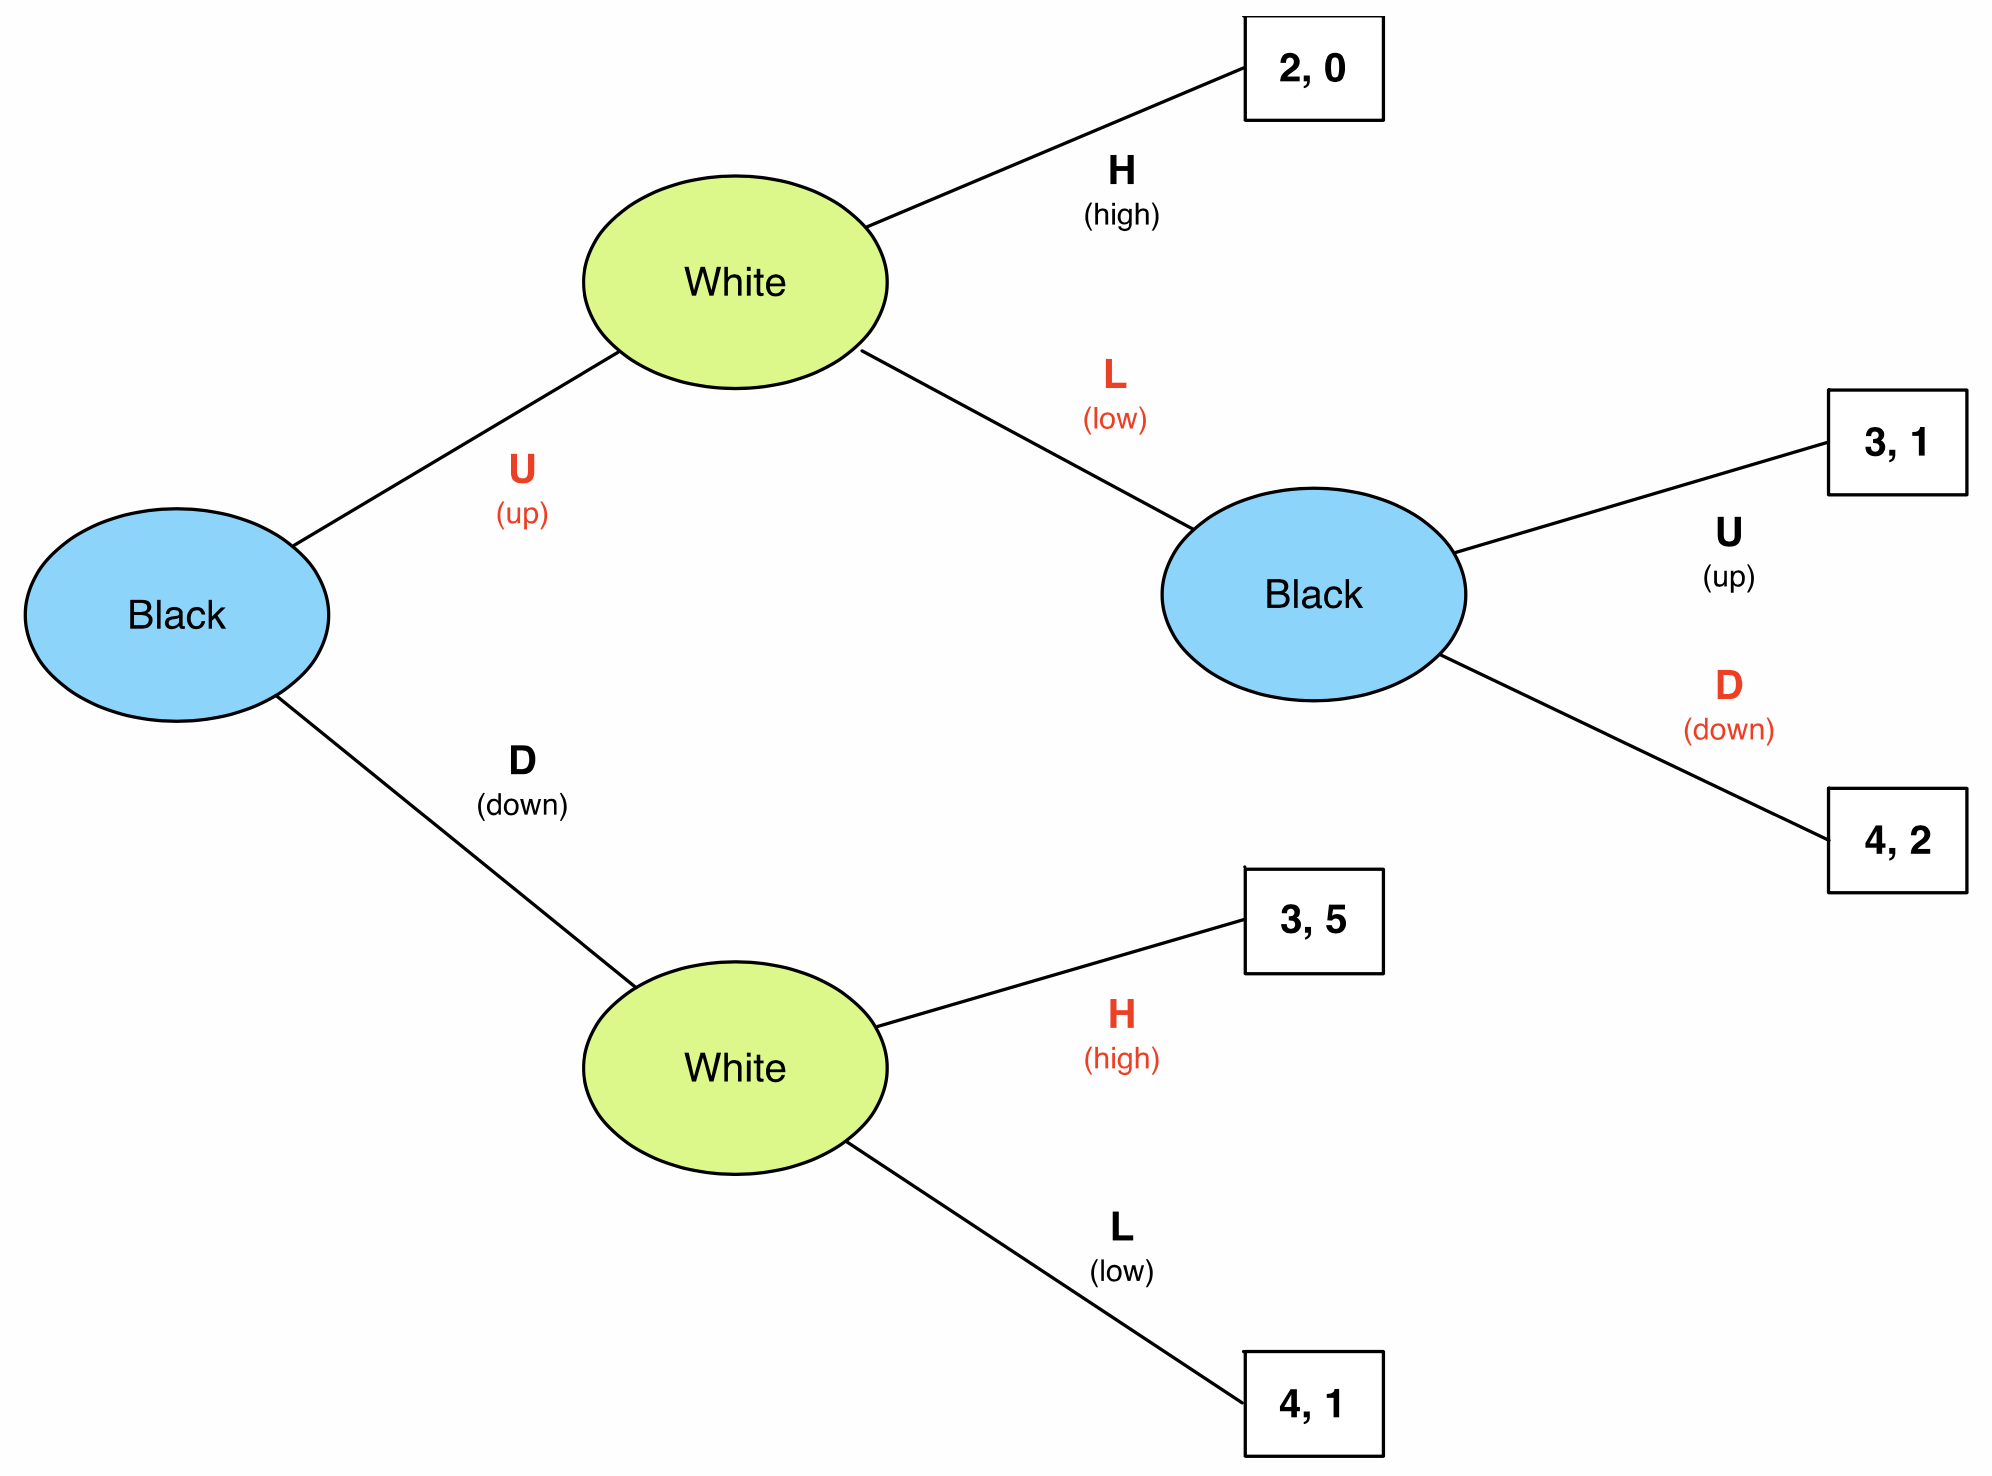
\includegraphics[width=0.45\textwidth]{img/backward_induction.png}
		\end{figure}
		
		\subsection{Wie funktioniert der Minimax-Algorithmus?}
		
		\begin{itemize}
			\item Wenn der Knoten mir gehört: Aktion wählen, die den Payoff maximiert
			\item Wenn der Knoten dem Gegner gehört: Aktion wählen, die den Payoff minimiert
			\item Wenn es ein Endknoten ist: Den Payoff berechnen
		\end{itemize}
		
		\subsection{Was ist die Formel für UCB1?}
		
		$U_{i} = \frac{W_{i}}{N_{i}} + c \sqrt{\frac{\ln N_{p}}{N_{i}}}$
		
		\vspace{1em}
		
		\begin{itemize}
			\item $W_{i}$ = Anzahl Gewinne mit der Maschine $i$
			\item $N_{i}$ = Anzahl Versuche mit der Maschine $i$
			\item $N_{p}$ = Anzahl Versuche insgesamt
		\end{itemize}
		
		\subsection{Erklären Sie den Algorithmus, der 1997 im Schach gewonnen hat.}
		
		\textbf{Deep Blue}
		\begin{itemize}
			\item 8000 handgefertigte Features
			\item Evaluation des Bretts mit dem Skalarprodukt zwischen Features und Gewichten
			\item Gewichte wurden vor allem von Hand angepasst durch menschliche Experten
			\item High-Performance parallele Minimax mit Alpha-Beta Pruning
			\item 480 spezialgefertige VLSI Schach-Prozessoren
			\item Durchsucht 200 Millionen Positionen pro Sekunde
		\end{itemize}
		
		\subsection{Wie heissen die 4 Phasen bei MCTS und wie würden diese aussehen?}
		
		\begin{figure}[htb!]
			\centering
			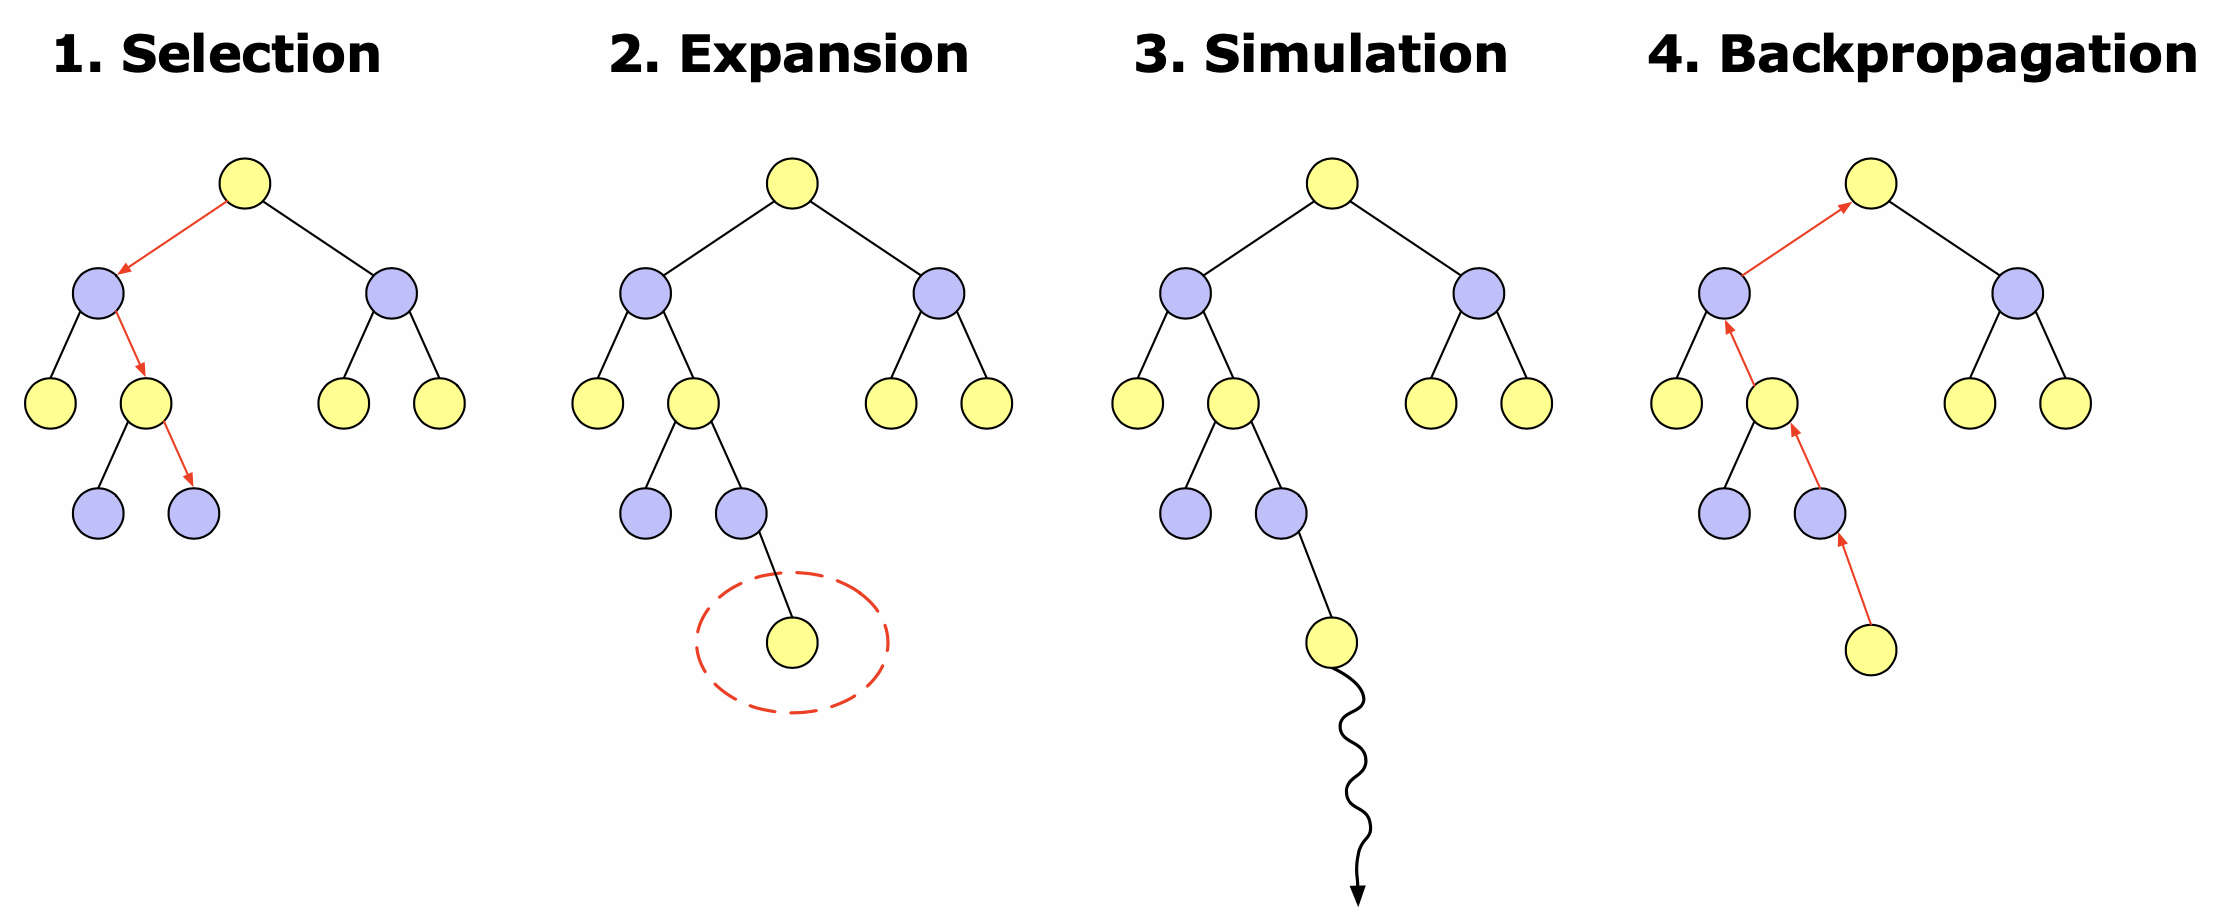
\includegraphics[width=0.7\textwidth]{img/mcts_phasen.png}
		\end{figure}
		
	
\end{document}
